\section{Example of an intrinsic RenderScript kernel usage}
\label{app:ex1}
\noindent Suppose we want to apply a Gaussian blur to a Bitmap image. Since Android gives an intrinsic script to implement this task we don't have to write a RenderScript file.

Here is the auto-esplicative code to use on Java side in order to correctly utilize Android API.

\begin{lstlisting}[frame=single]

// Create a Context
RenderScript mRS = RenderScript.create(this);

// Create a RenderScript Allocation to hold the input image.
Allocation inputAllocation = Allocation.createFromBitmap(mRS, myInputBitmap,
	Allocation.MipmapControl.MIPMAP_NONE,
	Allocation.USAGE_SHARED |
	Allocation.USAGE_GRAPHICS_TEXTURE |
	Allocation.USAGE_SCRIPT);

// Create an output Allocation, notice the USAGE flags are different
Allocation outputAllocation = Allocation.createFromBitmap(mRS, myOutputBitmap,
	Allocation.MipmapControl.MIPMAP_NONE,
	Allocation.USAGE_SHARED |
	Allocation.USAGE_SCRIPT);

// RenderScript has built in support for Blur so use that
ScriptIntrinsicBlur mBlur;

// First, we need to create the intrinsic
mBlur = ScriptIntrinsicBlur.create(mRS, Element.U8_4(mRS));

// And now we configure the intrinsic to perform our blur
mBlur.setRadius(20.f);
mBlur.setInput(inputAllocation);

// Now run the blur
mBlur.forEach(outputAllocation);

// Copy the output to our bitmap if necessary
outputAllocation.copyTo(myOutputBitmap);


\end{lstlisting}
\vspace{4ex}
And this is our image before and after the filter application:

\begin{figurehere}
 \centering
 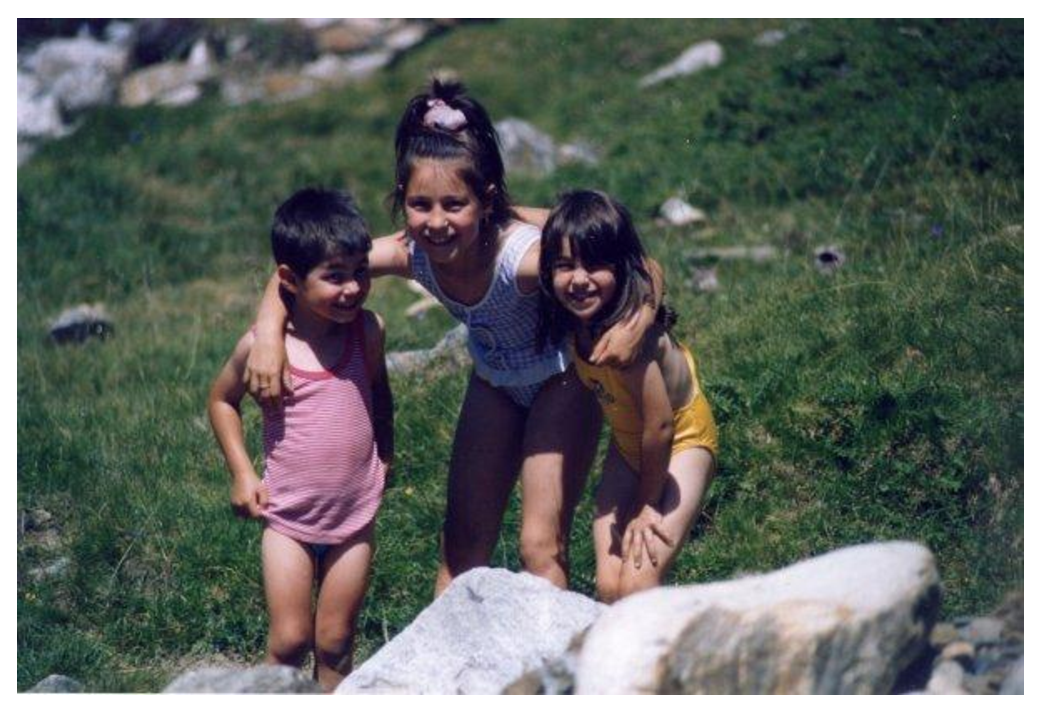
\includegraphics[width=0.5\textwidth]{./pictures/childhood}
 \label{fig:childhood}
\end{figurehere}
\begin{figurehere}
 \centering
 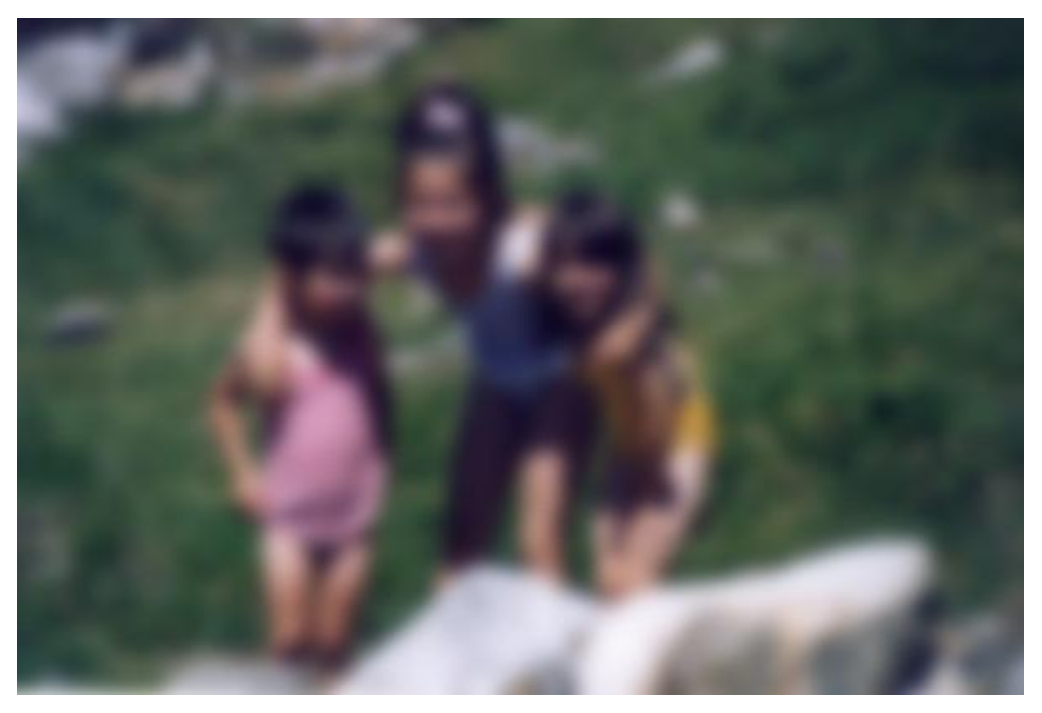
\includegraphics[width=0.5\textwidth]{./pictures/childhoodblur}
 \label{fig:childhoodblur}
\end{figurehere}

